\documentclass{acm_proc_article-sp}

\usepackage{graphicx}
 \usepackage{algpseudocode}
\usepackage{algorithmicx}
\usepackage{algorithm}
%\usepackage{algorithm2e}
\usepackage{amsmath}
\usepackage{amssymb}
\usepackage{amsbsy}
\usepackage{subfigure}
%\setcounter{tocdepth}{3}F4
\usepackage{multirow}
\usepackage{mdwmath}
\usepackage{mdwtab}


\begin{document}

\title{A distributed backbone-based framework for live video sharing in VANETs}
%\subtitle{[Extended Abstract]
%\titlenote{A full version of this paper is available as
%\textit{Author's Guide to Preparing ACM SIG Proceedings Using
%\LaTeX$2_\epsilon$\ and BibTeX} at
%\texttt{www.acm.org/eaddress.htm}}}
%
% You need the command \numberofauthors to handle the 'placement
% and alignment' of the authors beneath the title.
%
% For aesthetic reasons, we recommend 'three authors at a time'
% i.e. three 'name/affiliation blocks' be placed beneath the title.
%
% NOTE: You are NOT restricted in how many 'rows' of
% "name/affiliations" may appear. We just ask that you restrict
% the number of 'columns' to three.
%
% Because of the available 'opening page real-estate'
% we ask you to refrain from putting more than six authors
% (two rows with three columns) beneath the article title.
% More than six makes the first-page appear very cluttered indeed.
%
% Use the \alignauthor commands to handle the names
% and affiliations for an 'aesthetic maximum' of six authors.
% Add names, affiliations, addresses for
% the seventh etc. author(s) as the argument for the
% \additionalauthors command.
% These 'additional authors' will be output/set for you
% without further effort on your part as the last section in
% the body of your article BEFORE References or any Appendices.

\numberofauthors{6} %  in this sample file, there are a *total*
% of EIGHT authors. SIX appear on the 'first-page' (for formatting
% reasons) and the remaining two appear in the \additionalauthors section.
%
\author{
% You can go ahead and credit any number of authors here,
% e.g. one 'row of three' or two rows (consisting of one row of three
% and a second row of one, two or three).
%
% The command \alignauthor (no curly braces needed) should
% precede each author name, affiliation/snail-mail address and
% e-mail address. Additionally, tag each line of
% affiliation/address with \affaddr, and tag the
% e-mail address with \email.
%
% 1st. author
\alignauthor Mario De Felice\\
       \affaddr{University of Roma Sapienza}\\
       \affaddr{Rome, Italy}\\
       \email{defelice@diet.uniroma1.it}
% 2nd. author
\alignauthor
Eduardo Cerqueira\\
       \affaddr{Institute of Technology, Federal University of Para}\\
       \affaddr{Belem, Brazil}\\
       \email{cerqueira@ufpa.br}
% 3rd. author
\alignauthor Adalberto Melo\\
       \affaddr{Institute of Technology, Federal University of Para}\\
       \affaddr{Belem, Brazil}\\
       \email{adalbertocmelo@gmail.com}
\and  % use '\and' if you need 'another row' of author names
% 4th. author
\alignauthor Mario Gerla\\
       \affaddr{UCLA}\\
       \affaddr{University of California, Los Angeles, USA}\\
       \email{gerla@cs.ucla.edu}
% 5th. author
\alignauthor Francesca Cuomo\\
       \affaddr{University of Roma Sapienza}\\
       \affaddr{Rome, Italy}\\
       \email{cuomo@diet.uniroma1.it}
% 6th. author
\alignauthor Andrea Baiocchi\\
       \affaddr{University of Roma Sapienza}\\
       \affaddr{Rome, Italy}\\
       \email{baiocchi@diet.uniroma1.it}
}
% There's nothing stopping you putting the seventh, eighth, etc.
% author on the opening page (as the 'third row') but we ask,
% for aesthetic reasons that you place these 'additional authors'
% in the \additional authors block, viz.
%\additionalauthors{Additional authors: John Smith (The Th{\o}rv{\"a}ld Group,
%email: {\texttt{jsmith@affiliation.org}}) and Julius P.~Kumquat
%(The Kumquat Consortium, email: {\texttt{jpkumquat@consortium.net}}).}
\date{5 July 2014}
% Just remember to make sure that the TOTAL number of authors
% is the number that will appear on the first page PLUS the
% number that will appear in the \additionalauthors section.

\maketitle
\begin{abstract}
Vehicular Ad-Hoc Networks (VANETs) have been expanding their portfolio to support a large variety of services, ranging from safety to on-road multimedia applications. The distribution of real-time videos in a Vehicle-to-Vehicle (V2V) fashion allows drivers, passengers, paramedics, and first responder teams to capture, share, and watch video sequences from accidents and disasters that happened kilometers away. In this context, the transmission of live video streams in V2V scenarios must be done with Quality of Experience (QoE) criteria. This paper introduces the DBD (Distributed Beaconless Dissemination) protocol that improves the delivery of real-time video flows on multimedia highway VANETs, where it is important to maintain backbone-based routes for video dissemination in multi-path opportunistic V2V environments. The proposed solution improves the IEEE 802.11p MAC layer to solve the Spurious Forwarding problem, while increasing the packet delivery ratio and reducing the forwarding delay, especially in heavy vehicular traffic conditions caused by accidents, that we recreated from empirical data. Performance evaluation results show the benefits of DBD compared to existing works in forwarding video sequences in V2V VANET scenarios, on the basis of objective and subjective QoE  measurements.
\end{abstract}

% A category with the (minimum) three required fields
\category{C.2.1}{Network Architecture and Design}{}
%A category including the fourth, optional field follows...
\category{H.5.1}{Multi-media Information Systems}{}
%\terms{Theory}
\keywords{Vehicular Ad Hoc Networks, multimedia, QoE, safety, smart service}

\section{Introduction}
\label{intro}

The dissemination of live video flows over Vehicular Ad-Hoc Networks (VANETs) is becoming a reality, allowing passengers to have new experiences with on-road video flows \cite{Huang}\cite{Puangpronpitag2013}. Many vehicles are now equipped with video cameras and multimedia displays for different purposes, including monitoring and surveillance applications. However, most of the multimedia services are not used on-line. Many drivers around the world have installed video cameras in their vehicles for safety and surveillance applications. The automotive industry has also been developing vehicles with video cameras and radars, where the latter can detect suspicious objects and trigger video camera recordings.

Live video streams can be transmitted in a multi-hop Vehicle-to-Vehicle (V2V) fashion and provide users and authorities (e.g., first responder teams) with more precise information than simple text messages and allow them to determine a suitable action, while reducing human reaction times \cite{Vehicularcommunications:emergency}. Vehicles can cooperate with each other to share videos and show drivers, passengers, and first responder teams dangerous situations (videos) in both urban and highway scenarios.

Notice that the perception of multimedia content transmitted in VANETs and watched by humans, characterized in terms of Quality of Experience (QoE), is directly measured by the acceptability of the users and is related to, but differs from the extensively studied concept of Quality of Service (QoS) \cite{QualityEstimator}. QoS-based approaches and metrics, such as the ones based on link/network-related parameters  (e.g., packet loss and packet delay) fail to capture subjective aspects of video content related to human visual system that are essential in human-centric environments. Therefore, QoE metrics, such as Structural Similarity (SSIM) must be used to measure the video quality level from the user point-of-view \cite{QoEMu}.

The delivery of live short or long video sequences with QoE assurance in a V2V VANET environment is strongly influenced by forwarding schemes, especially in long distance transmissions and especially when the vehicle densities are very high like in the present paper, where an accident situation with high degree of congestion is considered. Besides the challenging scenario, the video flow must be disseminated to destination vehicle(s) placed kilometers away from the source (in a highway environment) and with a good quality level through V2V forwarding. Several forwarding solutions have been proposed in the literature for VANETs, where more details can be found in \cite{VehicularAdHocGerla}.

Contention-based routing has been attracting the attention of the VANET communities and allowing the dissemination of video flows in dynamic VANETs, where end-to-end routes may not exist all the time \cite{VideoBackboneDiFelice}. Proactive forwarding schemes choose the forwarder nodes before the content transmission, which is not suitable for dynamic scenarios as expected in many VANET environments. Contention-based reactive schemes decide the next-hop forwarder based on a distributed contention phase, which includes an extra delay in the selection process. In this context, to improve the performance of VANETs in delivering video sequences and video quality level, an opportunistic and beaconless geographic routing protocol is needed. A beaconless geographic routing protocol can define and maintain a high quality backbone for video sequences, while enhancing the packet delivery ratio and the quality level of video sequences, reacting well to dynamic scenarios, and avoiding the Spurious Forwarding (SF) problem \cite{VTCDeFelice}.

SF was introduced in \cite{VTCDeFelice} and it basically increases the number of forwarding nodes (clearly reducing the available bandwidth) and as the bitrate raises, it also brings to the interruption of the dissemination process, because of the wrong interpretation of the \textit{Inhibition Rule} (IR), which stops the forwarding operation by nodes that receive a packet, if they already received another copy of the same packet (that means that there is already another node in their transmission range who forwarded the packet). This rule generally applies to all the algorithms that have a distributed contention to elect the forwarding node.

To improve the delivery of live video flows on multimedia highway VANETs, this paper proposes the Distributed Beaconless Dissemination (DBD) forwarding scheme  together with an application framework that allows vehicles to seamlessly share videos in a certain area. DBD works on a multi-path environment and disseminates videos with a better quality from the human point-of-view. DBD aims to create and maintain V2V backbones for fast video packet relaying, thus increasing the packet delivery ratio, reducing the forwarding delay caused by the contention phase of reactive geographic forwarding schemes, and enhancing user perception when watching live video sequences. At the same time, it also aims to improve the IEEE 802.11p MAC layer utilization to solve the SF problem. The impact and benefits of DBD compared to existing geographic-based forwarding schemes for disseminating video flows in infrastructureless VANETs are presented with simulation and real QoE experiments.

The remainder of the paper is structured as follows. Section \ref{related} describes the related works; our proposal is explained in Section \ref{proposal}. Section \ref{performance} presents the test environment, scenario, implementations, and simulation results. The conclusion and future work are described in Section \ref{conclusion}.


\begin{figure*}[!thb]
\begin{center}
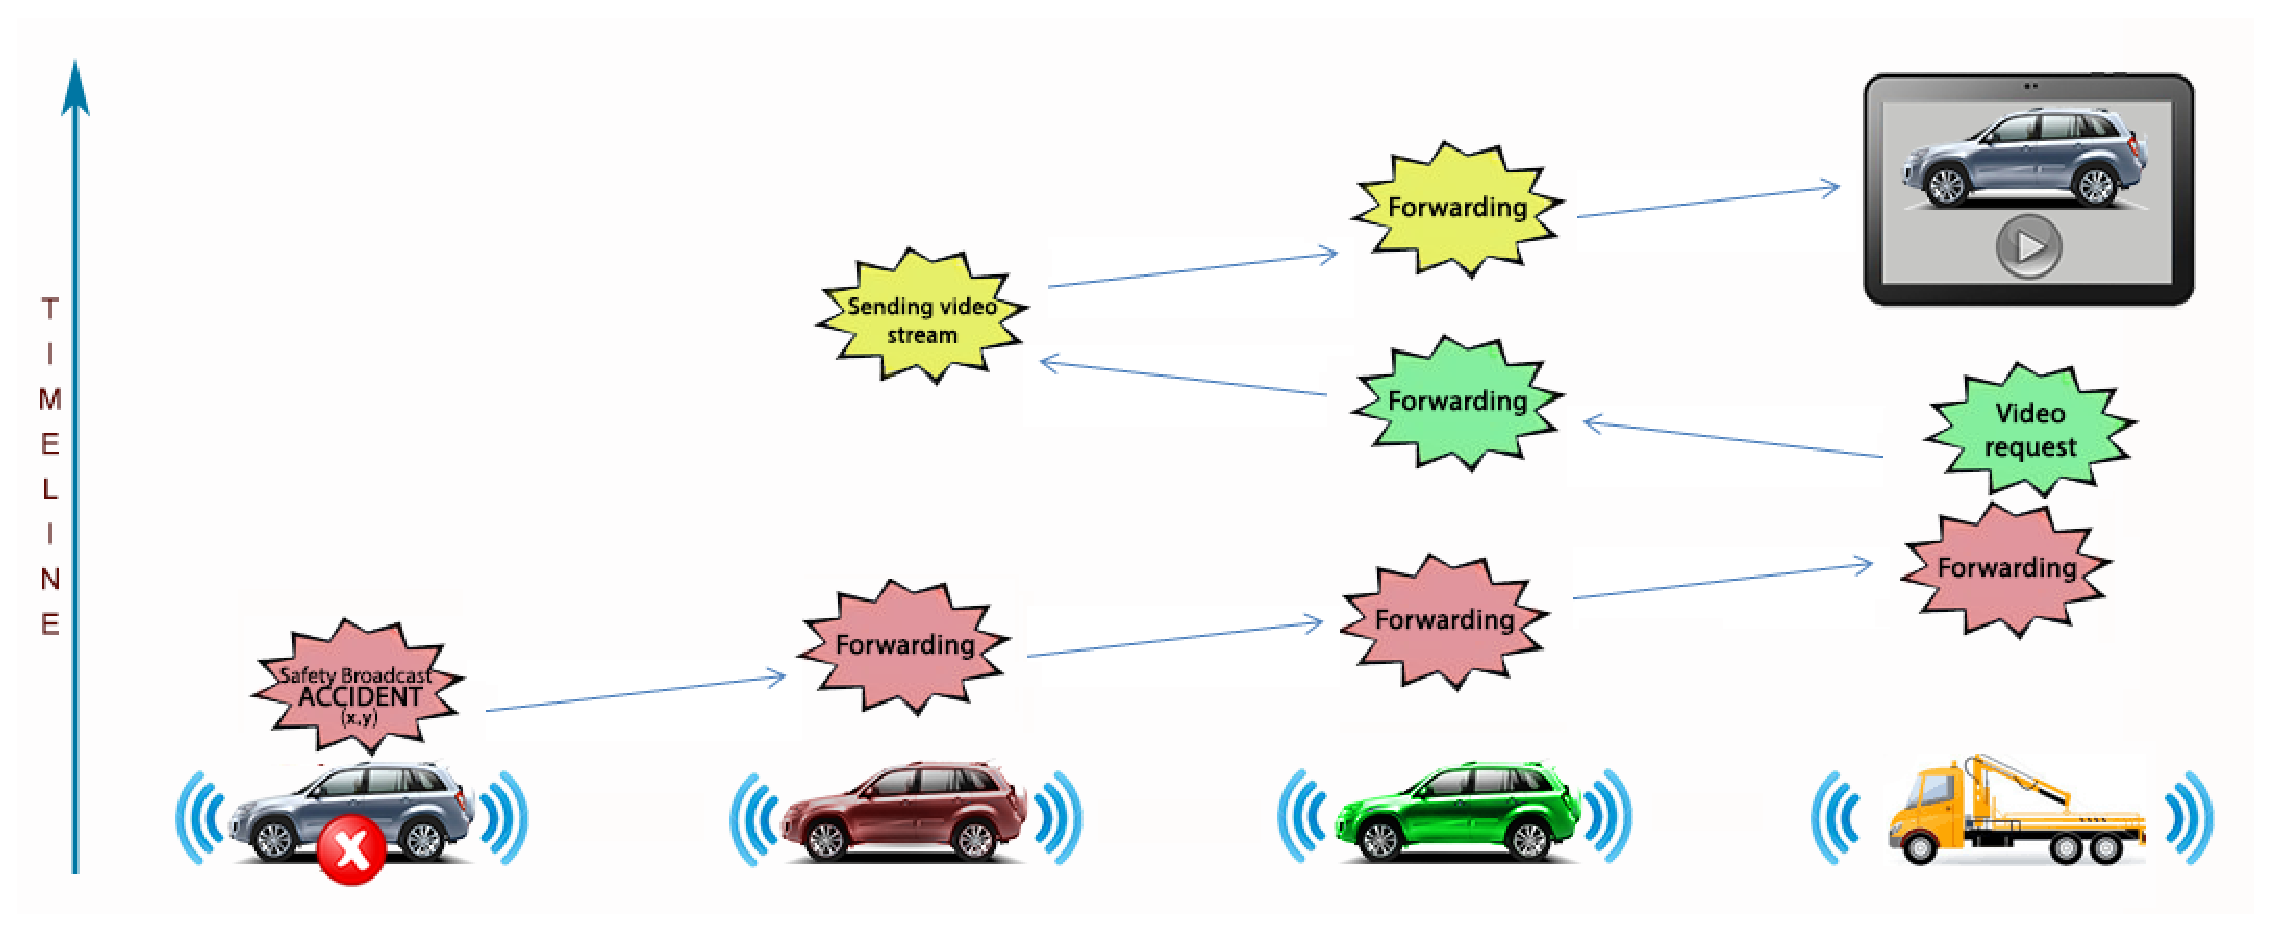
\includegraphics[width=1.5\columnwidth]{./fig/NewBigPicture.eps}
\caption{An example of our framework. After the safety packet, a video of the disaster is requested and then received by the requesting node}
\label{fig:bigpicture}
\end{center}
\end{figure*}


\section{Related Work}
\label{related}

A key approach to deliver video flows in VANETs is to use a reactive beacon approach, where such routing protocols select the next-hop relay through a distributed contention phase. However, this contention phase adds an extra delay in the system to decide the best forwarder vehicle.
An example of a reactive routing approach is proposed in \cite{torres2014v2x}, where Authors introduced two approaches for video transmissions in VANETs, both based on beacons. The former chooses the next hop with a delay-based logic (the farthest node forwards after the shortest timer), where beacons are used to exchange coverage information, (e.g. if a node receives a packet from another node that is known to provide more coverage area, it stops rebroadcasting that packet), the latter, in contrast, chooses the next hop as the node with more 1-hop neighbors. The impact of the logics on the video quality level, in any case, should be measured by QoE metrics (e.g., SSIM).

To optimize content distribution, a game theory-based scheme  (coalition formation algorithm) for video dissemination was proposed in \cite{MultimediaGameTheory}. The approach is promising, but the authors only dealt with a limited number of nodes and without QoE assessment, thus, it is not possible to identify the benefits of the proposed solution from the user point-of-view.

Besides the adopted approach, a basic requirement for multimedia content dissemination in VANETs, where the traffic pattern is very dynamic and unstable, is to create a dynamic relay nodes backbone, like in \cite{rezende2014receiver}. The Authors use a backbone based approach with a separate nodes election phase before the sending operation, based on a sophisticate distance-based rule in order to tackle the broadcast storm problem \cite{StormNew}. Even in this case, no QoE evaluation was performed. Moreover, lower layer problems, such as SF (Spurious Forwarding) were not considered.

Another backbone-based hybrid geographic routing for video sharing in VANET is presented in \cite{VideoBackboneDiFelice}. The Authors build a backbone and include several features in their design: the nodes election is delay-based and it accounts for vehicle speed and direction similarities in order to keep the backbone operative as long as possible. This approach uses beacons and ACKs. The study is interesting, especially because of the diverse application considered. The protocol suffers of significant operational overhead and, like the other backbone based protocols, does not consider SF in the selection.  Likewise, it does not evaluate the quality of the delivered videos based on QoE metrics.
Another backbone approach that may be interesting is \cite{medhocrubin}, where the Authors also use the knowledge of the lanes and the speed of the vehicles to elect a more stable backbone. The scheme is promising, especially when such a deep knowledge of the vehicles features is available. Such a scheme may be easily adapted to be used for video transmission, since its analysis is only focused on QoS generic performance.

One of the main differences of our protocol with respect to the other ones is the lack of beacons: our approach does not need them, nor any other additional mechanism is required to establish or maintain a backbone, nor to recover from failures.
At the MAC layer, most of the protocols have high error percentages at high bitrate, because they suffer from the SF problem \cite{VTCDeFelice}. Our solution solves it, thus providing lower loss ratios at high rates.
Another difference is the ROI (Region of Interest) feature: in our study, we cover a wider area through multi-hop (2-3 times bigger than in the other papers cited above) to ensure contact with emergency vehicles that may not be exactly close to the disaster scene. Bigger ROI is obtained thanks to the SF elimination (which causes a high probability of dissemination interruption, compatible with long lines caused by accidents). Moreover  we provide a higher number of vehicles and can handle higher densities in our study.
There can be other approaches for information dissemination in general, through probability or topology-based approach and more details can be found in \cite{dissemination}. However, the most important difference between our proposed scheme and the other ones is that in the latter video dissemination over a VANET is explored through standard network/packet metrics, without using good QoE metrics.








\section{The proposed application and \\routing framework}
\label{proposal}

This section introduces the proposed application framework and the DBD routing protocol for live video streaming in multi-hop VANETs, plus its interaction with the MAC layer to solve the Spurious Forwarding (SF) problem and improve wireless usage. The final aim is to share contents with authorized emergency vehicles/peers that can be located km away.

At the application level, the operation is pretty simple: by looking at Fig. \ref{fig:bigpicture}, when a vehicle has an accident, the neighbor cars (if any) detect the accidents (from secondary sensors, say sudden deceleration, stop, pattern recognition on video camera, etc). When the car determines that there is a reasonable probability that an accident occurred, it sends an alarm (automatic safety packet in red) to neighbors (possibly including a still picture of the accident, showing its view of the accident). It may also (optionally) post the video on the web using LTE. Note that this alarm uses DSRC spectrum. It is imperative NOT to send the full video immediately, else the network may be hopelessly congested by vehicles that mistake a simple slow down for accident. By using the red flow, a backbone of relay nodes is created, so that the number of forwarding nodes is limited (details in Sec. \ref{DBD}) and a logical infrastructure becomes available for transmission. The vehicles that are inside the ROI, which is less than 5 km away from the incident (they check their distance from the sender of the alert), forward the alarm. Beyond 5 km, the video of the accident will be picked up from the web.

Authorized vehicles near the crash, upon receiving the alert, can request the video download, using an ICN type approach, ie they send a request to one or more of the vehicles that have advertised their videos. The request triggers a video stream delivery from the origin or from other nodes on the DSRC backbone. For example, suppose an emergency vehicle receives this alert within the ROI, and it prepares to intervene (even before  any 911 call is received). Now, our application gives the opportunity to the emergency vehicle to request the video(s) of the incident scene from the most appropriate view points. This video request (in green) is forwarded back through the backbone
and reaches the nodes with their camera turned on.
Only nodes with a good view of the accident are probed. Automatically, with no driver intervention, the selected
yellow stream is forwarded back to the emergency vehicle, that can evaluate the situation on the incident
scene in real time and understand how to intervene and if other resources or particular equipment are required.

It is important to notice that all the packets are geo-tagged with previous hop, originator and/or destination/ROI coordinates, so direction of propagation is implemented. In particular the safety broadcast is sent in all the directions, while the other packets are forwarded only if they meet the direction criteria. For instance, a vehicle on the right of the ambulance, farther away from the accident would not forward the video request packet (the second message of the framework, after the safety one) on its right, because it knows its position, the position of the accident $x_{a},y_{a}$ (from the safety message) and the position of the source of the video request packet $x_{e},y_{e}$ (the emergency vehicle). Hence, it can build the logical ROI as a rectangle with diagonal equal to the segment from $x_{a},y_{a}$ to $x_{e},y_{e}$ and only forward the packet if it has to.

Since the packets travel in directional multi-hop (and thus broadcast) fashion, having more video requesters is not an issue, because the packet propagation is cut at the farthest destination, or propagated in more directions. For example, having an emergency vehicle in both directions of the highway simply means that the packet propagates both on the right and on the left of the source node. Moreover, having 2 emergency vehicles in the same direction implies that the packet's propagation is not interrupted at the first one, but at the farthest emergency vehicle: the ROI is calculated for the coordinates that maximize $d(x_{e,i},y_{e,i},x_{a},y_{a})$, where i represents the i-th emergency vehicle.

%Our proposal also wants to underline that, although in a shock situation, the driver only needs to push a single button: it is the only required action, thus the framework can be defined \textit{ automated}: the drivers do not really need to do anything but deciding about the quality of their video. Moreover, it does not need any LTE coverage (that may be missing in rural areas or highway). Through the VANET (Vehicular Ad-hoc NETwork), on a dedicated sub-channel of the spectrum, such video is propagated, so that the first responders can evaluate the current situation and directly assess the necessity to ask for further resources (an helicopter, a particular equipment) immediately and not only after they arrive at the accident location.

Our proposal can also be easily supported together with VANET ICN (Information Centric Networking) systems \cite{QualityEstimator}, where an event is announced and the requesting nodes ask for the content (Interest video flows).




%\subsection{How to solve the Spurious Forwarding problem at MAC layer}
%\label{spurious}
%
%This paper also proposes improvements in VANET MAC layer. So we identify and solve a problem that occurs at this layer: the Spurious Forwarding (SF) problem \cite{VTCDeFelice}. In order to understand the problem, we define the \textit{Inhibition Rule} (IR), which stops the forwarding by nodes that receive a packet, if they already received another copy of the same packet (that means that there is already another node in their transmission range who forwarded the packet). This rule generally applies to all the algorithms that have a distributed contention to elect the forwarding node.
%This mechanism may lead to problems in those cases where 2 forwarders win the contention in a very close time instant (comparable to the MAC service time). For example, we consider delay-based logic (the farthest away the node, the shortest the timer before forwarding) and by looking at Fig. \ref{fig:spurious}, when node A transmits its packet with sequence number $SN=k$, both $B$ and $W$ receive it and schedule the forwarding operation. $W$'s timer expires a moment before $B$'s one, so the channel is idle and it starts forwarding the packet. Meanwhile, $B$'s timer elapses, too, but since the channel is busy (although the packet by $W$ has not been received yet), $B$ is not inhibited and it schedules the forwarding operation at routing level. Once $B$ completes the reception of $W$'s packet, it finally understands there is no need by him to forward the packet but it is too late, since the packet has already been forwarded to the lower levels and now that the channel is free, the packet is sent a second time over the wireless medium. Any other node on the right with respect to $B$ and $W$, receives 2 copies of the packet with the same SN and inhibits itself (IR) because it thinks that a node in a better position than its, already took charge of the forwarding operation. Dissemination is thus interrupted.
%
%
%\begin{figure}[tb]
%\begin{center}
%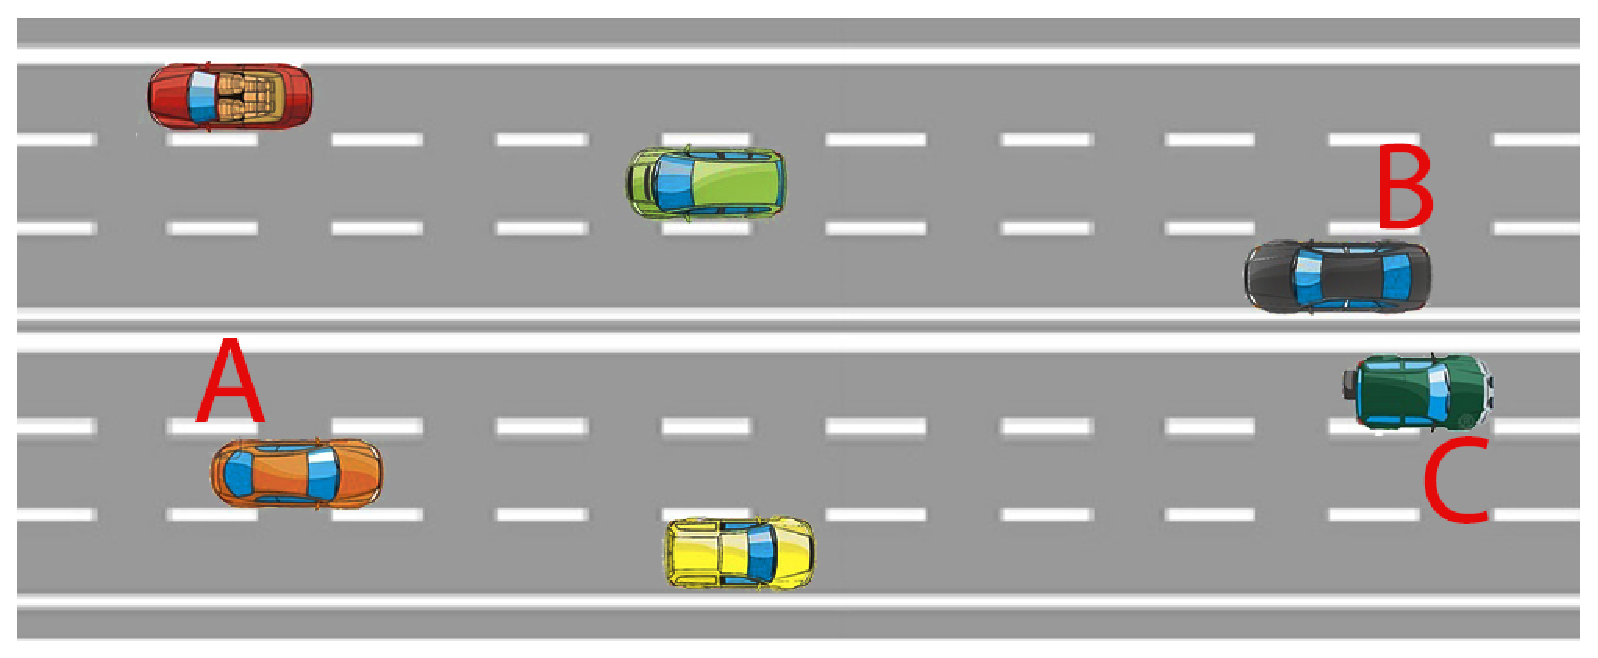
\includegraphics[width=.9\columnwidth]{./fig/newspurious.eps}
%\caption{An example of spurious forwarding}
%\label{fig:spurious}
%\end{center}
%\end{figure}

\begin{figure}[tb]
\begin{center}
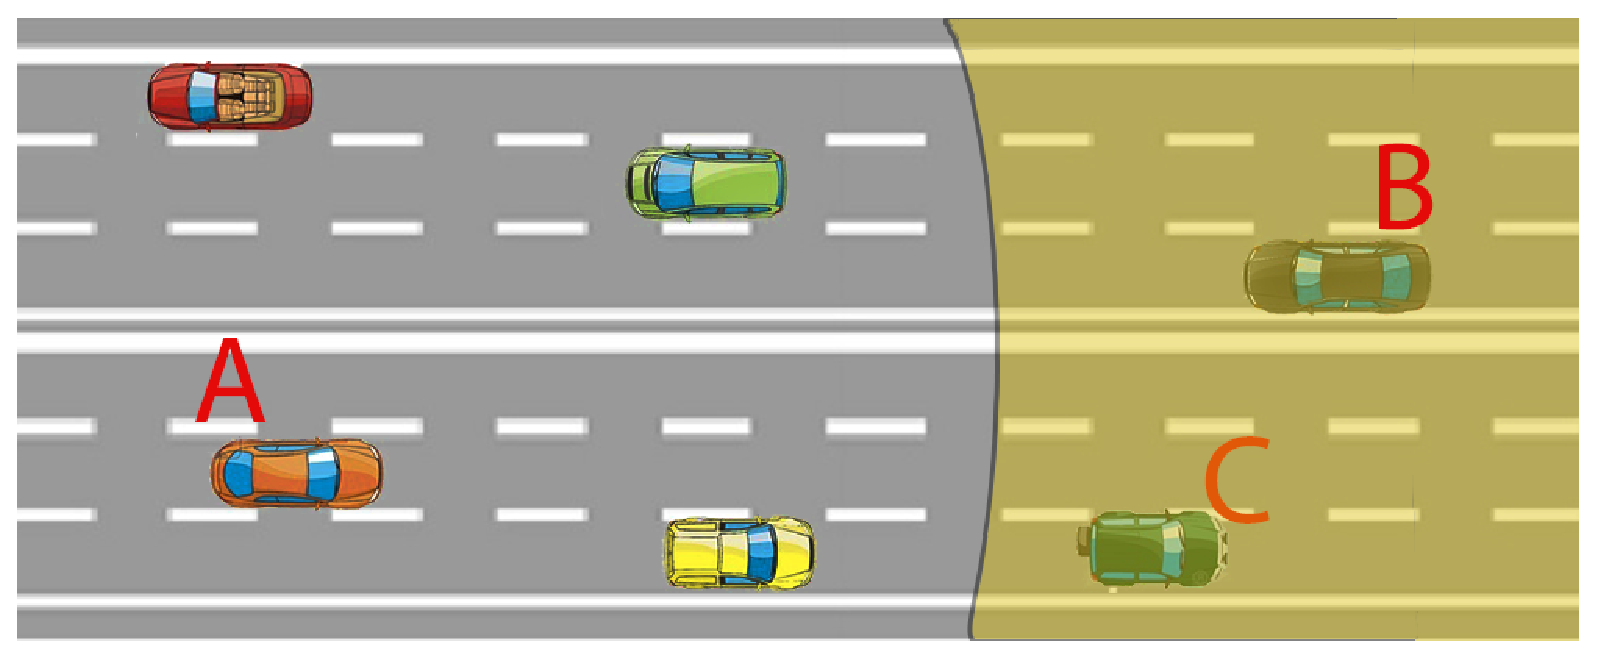
\includegraphics[width=.9\columnwidth]{./fig/CarreggiataNOc.eps}
\caption{If the node $A$ sends a packet, $C$ is going to be the forwarder. In yellow, it is possible to see the forwarding zone in which DBD elects the \textit{BN}}
\label{fig:carreggiata}
\end{center}
\end{figure}



\subsection{The backbone routing logic}
\label{DBD}

At a routing level, this protocol is designed with a precise aim: building an on-demand distributed backbone, with no overhead packets, no need for RSU or any other external information.
The rule to elect the backbone nodes is that when a node receives a packet, it starts the following timer:
\begin{equation}
\label{eq:timer}
T = T_{max} \left(1- \frac{d(v_{sender},v_{receiver})}{R_{max}}\right)
\end{equation}
where $R_{max}$ is the maximum transmission range and $T_{max}$ the maximum delay (the bigger, the more precise but slower the selection), such that $T$ is the shortest the farthest away it is from the sender, $v_{sender}$ and $v_{receiver}$ are the vehicles that, respectively, send and receive the packet. Who wins, forwards the packet, the other nodes are inhibited according to the \textit{IR} defined in sec. \ref{intro}.

\textbf{\textit{BN} election}. When the node $W$ wins the forwarding contention (because of its shortest timer), this means it is in the best position to forward the packet, thus it elects itself as \textit{BN} and sets its timer to 0 until $\alpha R_{max} \le d \le R_{max}$, where $\alpha \in (0,1)$, empirically evaluated and equal to 0.75 in our experiments. As a matter of fact, this implies that it exists a zone within the transmission range of every node which is considered \textit{forwarding zone}, as we can see in Figure \ref{fig:carreggiata}. In yellow, in fact, it is highlighted the portion of the transmission range where the \textit{BN}s are elected. If a \textit{BN} leaves it (by getting closer to the previous hop's \textit{BN} or by moving out of range), this triggers a new election for that node of the backbone.

\textbf{Self-repairing}. If the \textit{BN} moves out of the \textit{forwarding zone} or fails, since the other nodes still keep their timers running, a new \textit{BN} is elected in at most $T_{max}$. This mechanism distributely grants resilience to the protocol, and by changing the parameter $\alpha$, it is possible to have a more stable backbone with a sub-optimal position of the hops (and most likely a greater number of hops) or, at the opposite, getting an extremely tuned backbone, but with a shorter life and more hardly elected. The extreme example is for $\alpha=1$, where only if there is a node exactly at distance $R_{max}$ from the sender ($A$ in the figure), a \textit{BN} is elected; otherwise the packet is forwarded, but without the permanent election of the \textit{BN}.

\textbf{Buffer transmission}. When a \textit{BN} is elected, it transmits all its other enqueued packets waiting for the timer to expire. There is no need to wait further, since if the \textit{BN} has just been elected, it is certainly in the best position to forward all the packets that it can forward.

\textbf{Spurious Forwarding elimination}. In order to solve the SF problem introduced in sec. \ref{intro}, we introduce a Hop Count (HC). In fact, if 2 vehicles $F$ and $G$ have a very similar timer, such that it is less than the MAC service time, they will both schedule the forwarding operation, but when $F$ and $G$ receive the message copies they have forwarded, carrying the same HC value, they check their distance with respect to the sender of the previous hop, so they autonomously consider themselves not \textit{BN}, if their distance from the previous hop is less than the one in the message they received. This implies that automatically and without any other overhead message, one node between $F$ and $G$ revokes itself the \textit{BN} status, thus preventing the SF to happen again until the best \textit{BN} stays in the \textit{forwarding zone}.
The same principles apply when multiple spurious forwarders are involved. Besides the HC introduction that avoids dissemination interruption, this solution eliminates the problem and allows higher rates transmission, because the channel is not uselessly overloaded.

\textbf{Direction Control}. In order to keep the backbone in place as long as possible, it is better to choose the backbone nodes traveling in the same direction. This allows to keep the inter-vehicle distances within the $\alpha$ threshold, so that it happens less frequently that a \textit{BN} must be re-elected, maybe just because that specific \textit{BN} was travelling in the wrong direction, thus it went out of the \textit{forwarding zone} too fast. The direction is recognized by simply comparing the node's previous position and the current one (this happens for every packet reception or every 15 seconds, whatever comes first). As it is possible to see in Figure \ref{fig:carreggiata}, in fact, if $A$ is the previous hop's \textit{BN} and its \textit{forwarding zone} is the yellow one, the only node that can be chosen is $C$, because $B$ is travelling in the wrong direction, although it is in the \textit{forwarding zone}.

\textbf{Loop protection}. In urban scenarios (not simple highways), there could be loops that HC solves, even if it can take several unnecessary forwarding operations; in fact, let $h$ be the last HC number received for a given message with sequence number $k$. Let $h_{new}$ be the HC carried by a second received copy of the message with sequence number (SN) $k$. The \textit{IR} is triggered and both copies of the message are no more considered for forwarding if $h_{new}<h$, which means that if $h_{new}$ is smaller that $h$ and it is arrived later, then it cannot be arrived from previous hop vehicles, but from a loop, so it is discarded without any further operations.

\begin{algorithm}
\begin{algorithmic}
\If {SN not completely processed and correct propagation direction}
		\If {SN's first reception}
				\If {I am a BN}
					\If {I am in the \textit{forwarding zone}}
						\State \Call {send}{packet}
					\Else {} \Call{schedule forwarding}{packet}
				    \EndIf
			    \Else {} \Call{schedule forwarding}{packet}
			    \EndIf
		\Else {} \Call{hopcount processing}{packet}
	    \EndIf
\EndIf
\State
\Function {send}{packet}
    \State send packet and all the other ones waiting: I am a \textit{BN}
\EndFunction
\Function {hopcount processing}{packet}
	\State Check on $h_{new}$:
	\State $h_{new}<h$: loop protection
	\State $h_{new} \geqslant h + \gamma$: Remove my \textit{BN} status
	\State $h \leqslant h_{new} \leqslant h + \gamma$: Spurious Forwarding check
	\State Restart the esecution
\EndFunction
\Function{schedule forwarding}{packet}
			\State schedule forwarding and wait for it to elapse
			\If {no copies received} \Call{send}{packet}
			\Else {} \Call{hopcount processing}{packet}
			\EndIf
\EndFunction
\caption{the DBD pseudocode upon packet reception}
\label{alg:algorithm}
\end{algorithmic}
\end{algorithm}

After the explanation of the single features of this protocol, it is possible to analyse its behaviour when a packet with a sequence number $s$ arrives to a node. By following the algorithm \ref{alg:algorithm}, when a packet is received, if it was never completely processed before, the node checks if the direction is ok (e.g. if it is outside the ROI or if the propagation direction is correct). In case the check is ok, the node checks if the sequence number $s$ was already received once before. If the answer is affirmative, the node checks the packet's hop count $h_{new}$. If it is much greater than the one it has in memory ($h$), then the node should not consider itself as a \textit{BN} and end the processing.
In case $h_{new}<h$, instead, we are facing a packet from a loop, so the processing ends, too. The third option is if $h \leqslant h_{new} \leqslant h+\gamma$, where $\gamma$ is a constant greater than zero, equal to 3 (normally $gamma=1$ is ok, but the value of 3 adds robustness in case the packet with $h_{new}+1$ is somehow lost). In this case, we may be facing a spurious forwarder, so IR does not block the processing and it is the only case that makes the processing continue.

In fact, if this is the case, the node checks its backbone status: if it is a $BN$, then it checks if it is still in the forwarding zone ($\alpha R_{max} \le d \le R_{max}$). If the answer is affirmative, the packet is sent immediately (and possible pending messages are sent, too). In the other case, as happens for non-BNs, the node schedules a timer and when it elapses, if no other copies have been received, the packet is sent (and the node becomes BN).




%\begin{figure}[!t]
%\begin{center}
%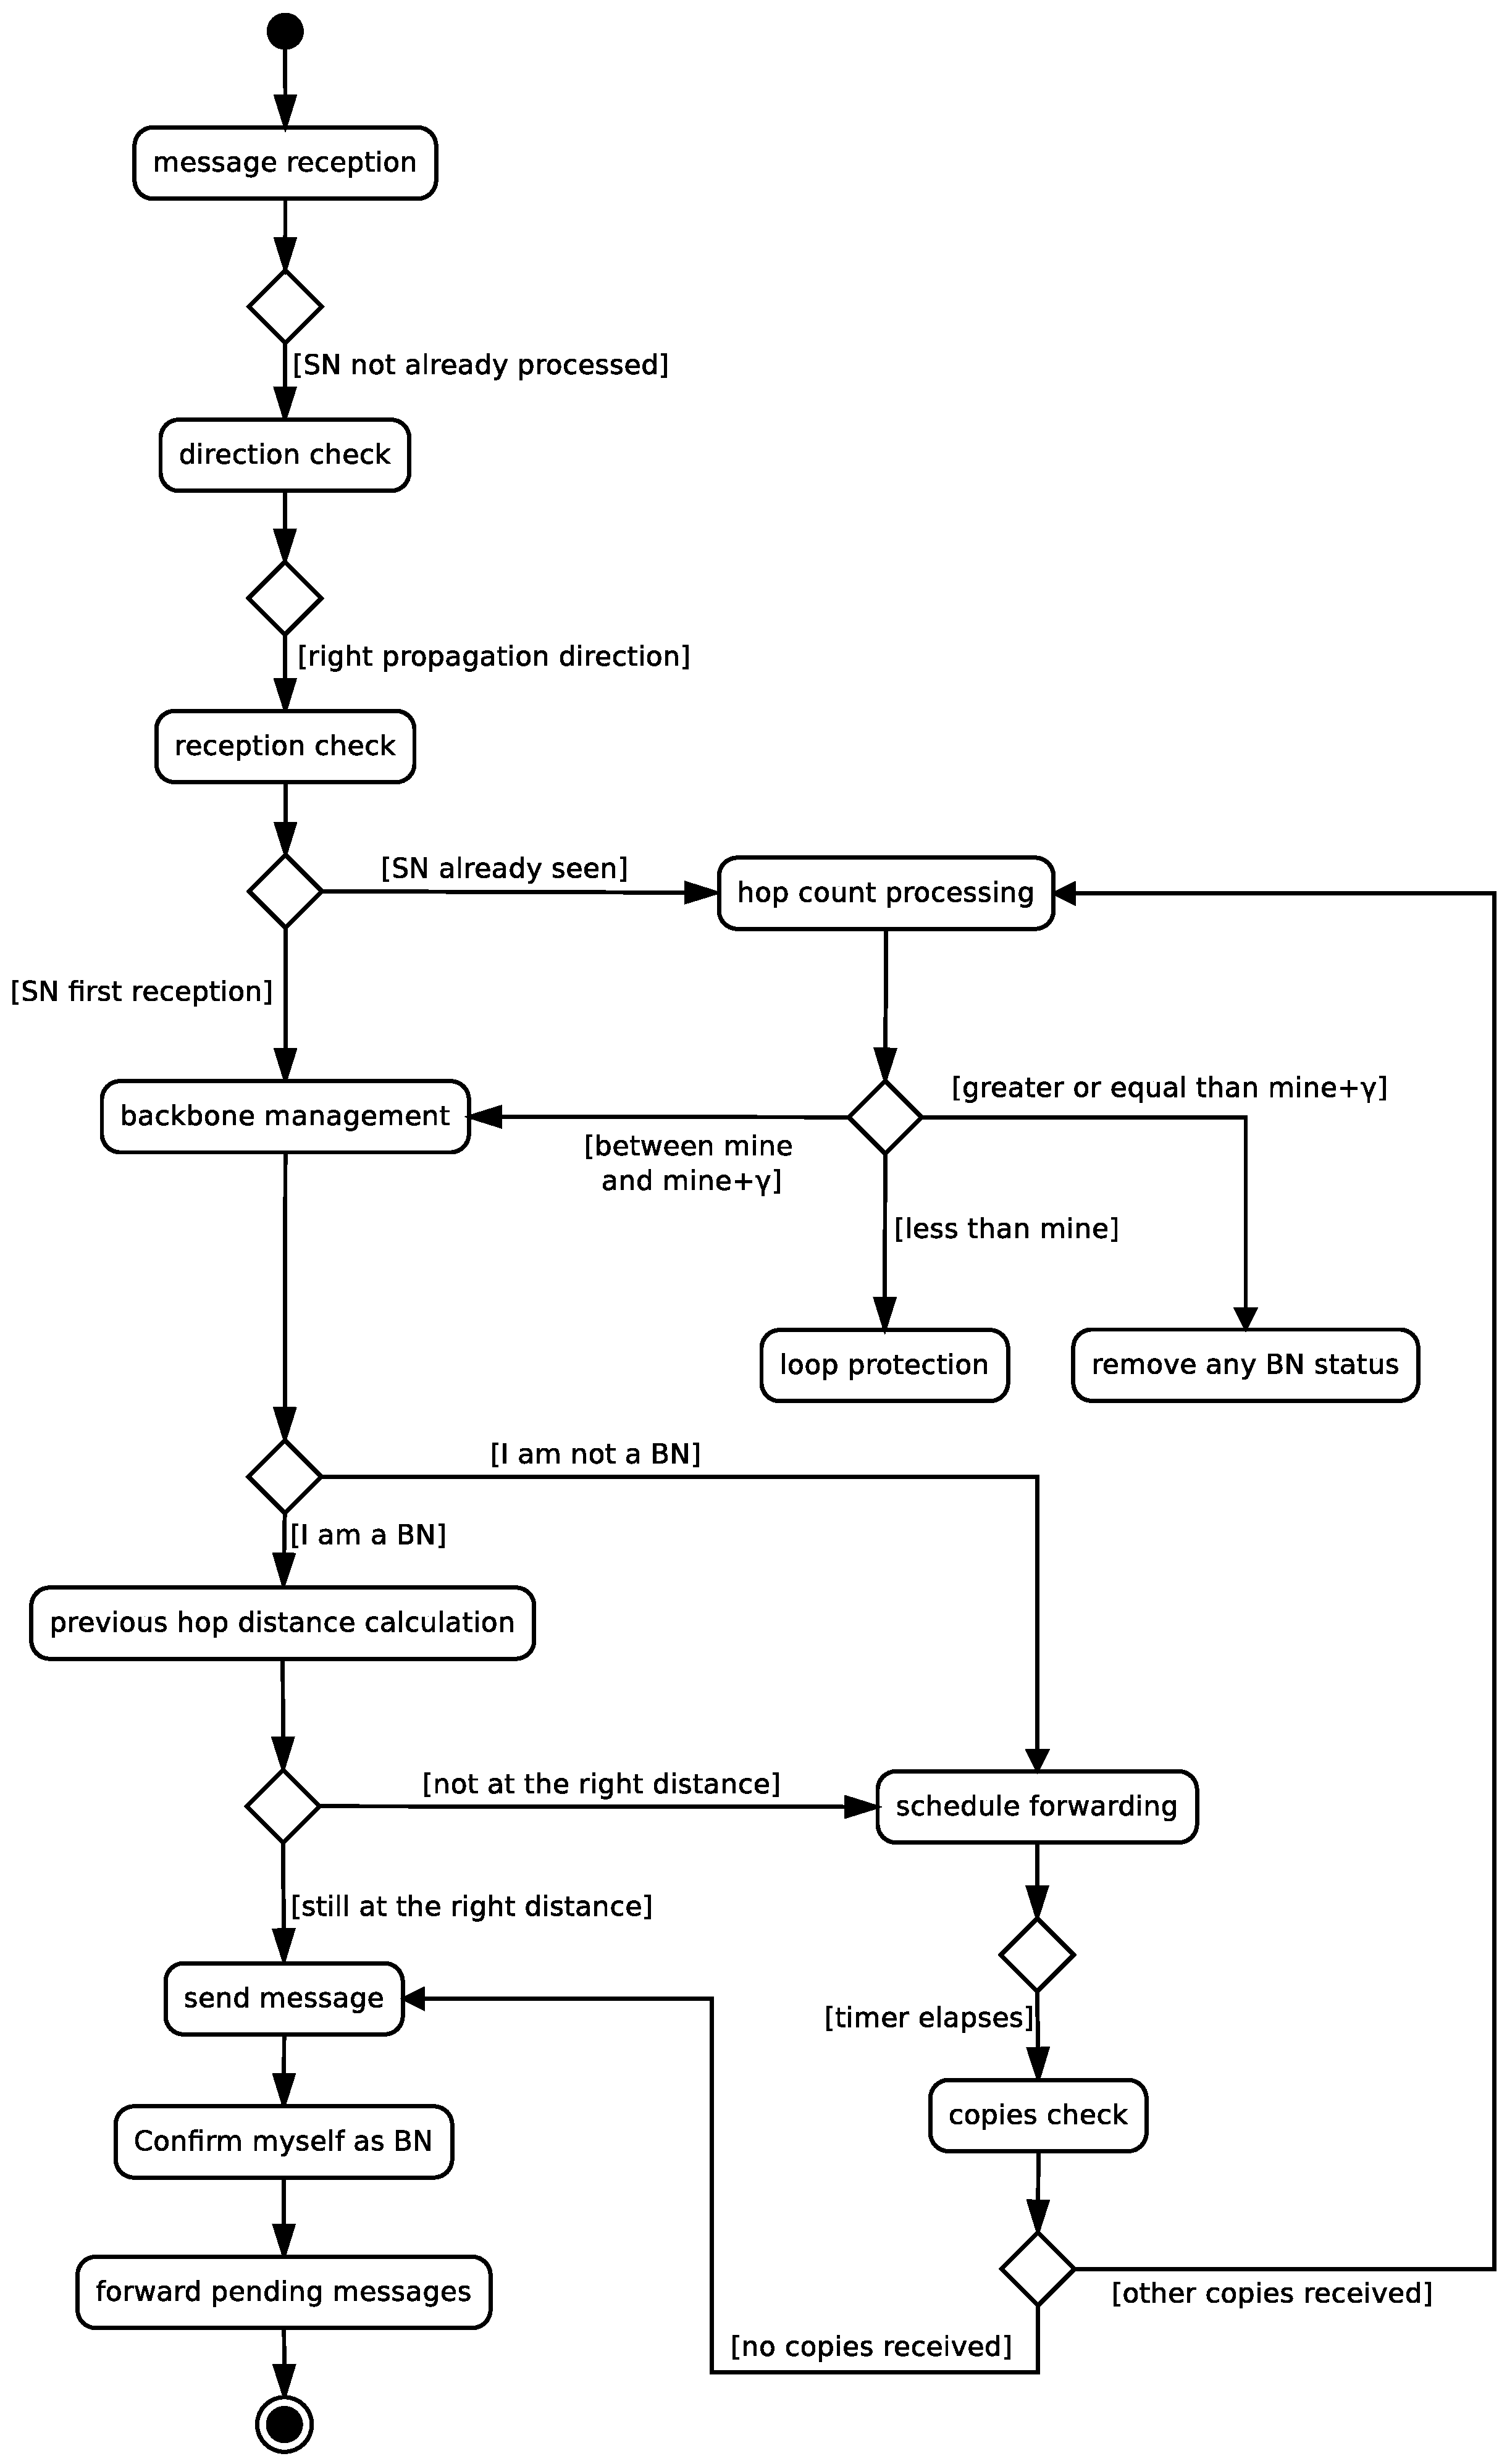
\includegraphics[width=.9\columnwidth]{./fig/Diagramma4.eps}
%\caption{Activity diagram of the node behavior after the reception of a message}
%\label{fig:flowchart}
%\end{center}
%\end{figure}




\section{Performance Evaluation}
\label{performance}

This section analyses the benefit and the impact of DBD in disseminating video sequences in highway VANET scenarios. It is done by measuring PDR (QoS) and SSIM (QoE) metrics. The DBD performance is compared to key forwarding proposals, namely DBF (Delay Based Forwarding) \cite{DDT}, PBF (Probability Based Forwarding) \cite{PBF}, and RND (Random Forwarding) \cite{RND}.  The aim is to cover the major nodes picking strategies, all of them providing IR, with a distributed beaconless approach, based on a timer or a probability started upon the reception of the first copy of a packet.

Notice that all the proposed protocols have been enhanced with respect to their originals. Thus, they are aware of the desired packet propagation direction and exploit it for the forwarding strategy. Moreover, we needed to equip all the protocols with a mechanism to reduce the forwarding contention timer: once a node successfully transmitted a packet in the flow, its timer for the next $s$ will be halved (or probability function doubled-up). We included these improvements because the standard protocols, as they were, provided too poor performance and did not represent a real comparison.
The examined protocols are:
\begin{enumerate}
	\item DBF: The farthest away the node, the shortest the timer \cite{DDT}.
	\item PBF: The closer the node, the lower the forwarding probability \cite{PBF}.
	\item RND: The thrown timer is a random number $T \in [0,T_{max}]$ \cite{RND}.
\end{enumerate}

\subsection{Methodology, Scenarios and Metrics}
\label{methodology}
To get realistic scenarios and results, the experiments were carried out by using a well-known real video sequence (named Akiyo), Evalvid Tool \cite{evalvid}, and real maps from open street map \cite{openstreetmap}, which were imported into SUMO (Simulation of Urban MObility) \cite{SUMO}, allowing us to generate the desired vehicle flows, with realistic behavior and vehicle-to-vehicle interactions. In addition, the VANET environment implements a car-following model together with random cruise speed and several vehicles classes, selected according to empirical data. In particular, in this paper we want to stress a situation where the traffic is very congested because of the accident that our application aims to stream to the emergency vehicles. We also imported a 8 km portion of the San Diego Freeway map that runs along the UCLA campus in Los Angeles. Furthermore, the video flow and the road/vehicle characteristics were integrated into Network Simulator 2 (NS2) \cite{ns2} together with the implementation of the forwarding schemes.

%\begin{figure}[tb]
%\begin{center}
%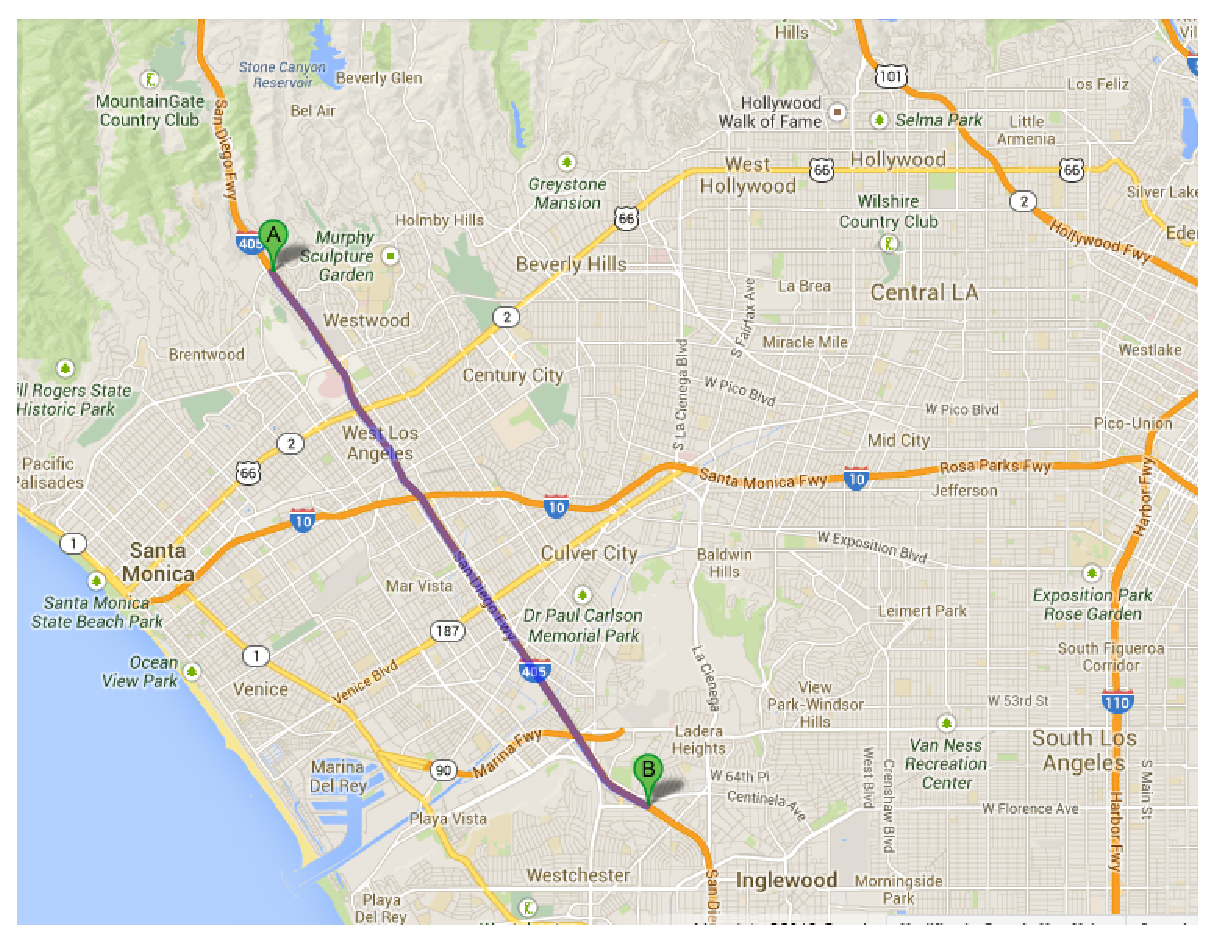
\includegraphics[width=.7\columnwidth]{./fig/map.eps}
%\caption{Simulation highway scenario}
%\label{fig:map}
%\end{center}
%\end{figure}

The simulator was configured to run 20 simulations in scenarios with different conditions. The vehicle density level on the roads is of 400 nodes per km and the distance between the source and destination $d(S,D)$ varies from 2 Km to 4 Km. The major simulation parameters are summarized in Table 1.
\begin{table}[b]
	\label{tab:parameters}
	\begin{center}
	%\subtable[Scenario and vehicular traffic parameters\label{tab:T1}]{%
	\begin{tabular}{l|l}
	\hline
	\multicolumn{1}{c|}{\textbf{Parameters}} &
	\multicolumn{1}{c}{\textbf{Values}} \\
	\hline
	$d(S,D)$, End-to-end distance (km) & 2, 4 \\
	Number of lanes per direction & 5 \\
	Vehicle max speed (km/h) & $130$\\
	Average total vehicle density (veh/km) & $400$ \\
	Video GoP length &  15\\
	Data rate (kbit/s) & $1000$  \\
	MAC, PHY parameters & IEEE 802.11p \\
	Propagation Model & Two ray ground \\
	Transmission Power (mW) & $500$ \\
	Max range ($R_{max}$ m) & $553$\\
	Max forwarding delay ($T_{max}$ ms) & $100$\\
	\hline
	\end{tabular}
	\caption{Simulation parameter values}
	\end{center}
	\label{tab:parameters}
\end{table}

In addition to QoS metrics (e.g., Packet Delivery Ratio, which is the ratio between the number of packets correctly received at the destination and the total sent packets), a key objective QoE metric, named SSIM, was used to show the impact of routing schemes on the user perception in scenarios with different node densities and end-to-end distances. The SSIM metric is based on original and processed video sequences and a frame-to-frame assessment of three video components, i.e., luminance, contrast, and structural similarity. It ranges from 0 to 1, and a higher SSIM value means better video quality. We used the MSU Video Quality Measurement Tool (VQMT)  to collect the SSIM values for the delivered video sequences.

It is important to highlight that the MPEG standard defines three frame types for the compressed video streams, namely I (Intra-coded), P (Predictive-coded), and B (Bidirectionally predictive-coded) frames. In a video sequence, I frames are the most important ones from the human point-of-view. The successive frames between two succeeding I frames define a Group of Pictures (GoP). A GoP pattern is characterized by two parameters as follows: GoP (N, M), where N is the I to I frame distance and M is the I to P frame distance. The encoding/decoding correlation between the frames, in particular, the B and P frames, depends on the respective preceding and succeeding I or P frames. For the experiments, the GoP length of the MPEG Akiyo video is of 15 and represents typical Internet-based videos. A total of 40 distorted video sequences were collected from the simulations (20 videos when the distance from the source to the destination is of 2 Km and 20 videos for 4 Km). All results are presented with a confidence interval of 95\%.




\subsection{Evaluation Results}
\label{Evaluation Results}
In order to compare our scheme with the other ones, we simulated the most challenging part of the framework: the video streaming phase (the yellow stream in Fig. \ref{fig:bigpicture}) and most important, our analysis depicts a worst case scenario, in fact, when the transmission starts, the DBD backbone is created on-the-fly, and the vehicles density is very high, thus facilitating collisions. This scenario illustrates typical problems in VANETs.




\subsection{QoS Results}
\label{QoSResults}

In Fig. \ref{fig:qos} we can see the PDR (Packet Delivery Ratio) per GoP in each video sequence. As we expect, because of Spurious Forwarding, DBF stays at about 10\% because after few hops and with such a high traffic density, it simply cannot overcome the spurious duplicates. RND, instead, because of the random timer, can overcome this problem in a better way, like PBF, since the spurious forwarders are not necessarily in the same, very limited, space frame (DBF chooses the forwarder among the farthest nodes from the sender), but they are better distributed on the road in such a way that the farthest nodes for every hop may not receive the spurious duplicate.

Moreover, the DBF, RND, and PBF protocols do not build a backbone, so they have to elect the forwarder node for every hop and for every packet. This slows down the whole mechanism and quickly leads to saturation of the available bandwidth and packets stack: packets to be forwarded start to pile up in the nodes until they start to be discarded; in fact, all the 3 slopes start at a higher point and then converge to a lower one. The final higher value is due to the fact that the buffer is being emptied without new packets incoming.
For this reason, when DBD starts (in our simulation, DBD starts without a backbone), it reaches a lower PDR with respect to its stationary point, because it has to build the backbone: if a previous flow has already been transmitted, this step is skipped. Once it builds it, then the PDR starts to rise and stabilize, queues are emptied and after GoP 5, it also goes on growing. In these conditions, with a dense scenario, which happens in case of highway incident, instead of suffering the presence of too many nodes to coordinate, it benefits from it.
When dealing with delay, DBF and RND take about 200ms (over the packet play-out deadline) to get to the destination (they are timer-based) and 100ms for PBF on the average. DBD, instead, just needs 20ms with the backbone in place. As a final consideration, the starting point (GoP=0) gives a hint about the impact of the SF problem alone, since none of the protocols has a backbone at that stage.


\begin{figure}[tb]
\begin{center}
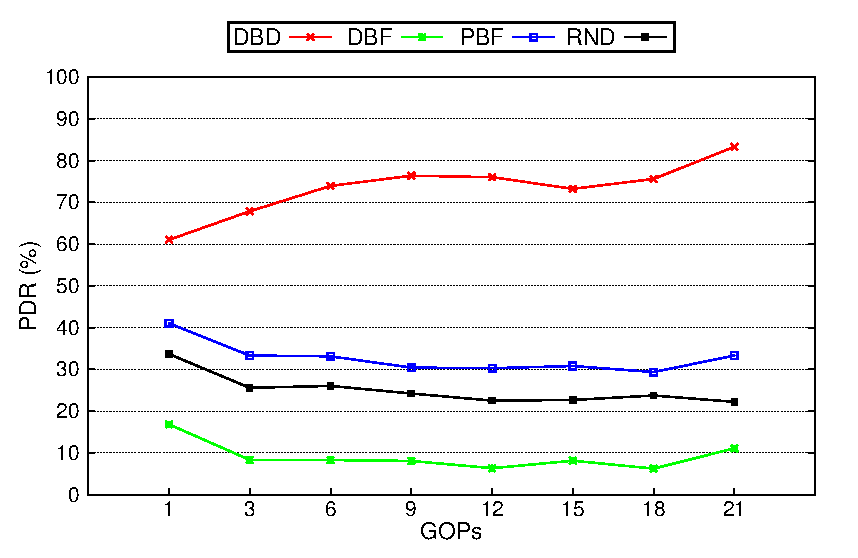
\includegraphics[width=.9\columnwidth]{./fig/selected/LinePDRxGOPIDfinal.eps}
\caption{Average PDR per GoP ID}
\label{fig:qos}
\end{center}
\end{figure}




\subsection{QoE Results}
\label{QoEResults}
This section shows the impact of disseminating video flows in VANETs by using SSIM. The SSIM metric measures the video quality level, by analyzing the frames based on their luminance similarity, contrast similarity, and structural similarity.
Figure \ref{fig:SSIM} shows the average SSIM results for video transmissions in all scenarios and when the system is configured with all the forwarding schemes. It is possible to see that DBD aims to keep the SSIM values over 0.7 at the beginning of the video transmission and over 0.8 after the backbone construction. Between GoPs 15 and 18, the SSIM results for the videos are reduced, because DBD needs to readjust the backbone. On the average, DBD increases the video SSIM by about 20\% compared to DBF, RND, and PBF. When the SSIM values are below 0.6, most of the videos cannot be displayed on the destination device or the quality is very poor that the scene cannot be watched by the end-users (see Fig. \ref{fig:POV}).



\begin{figure}[tb]
\begin{center}
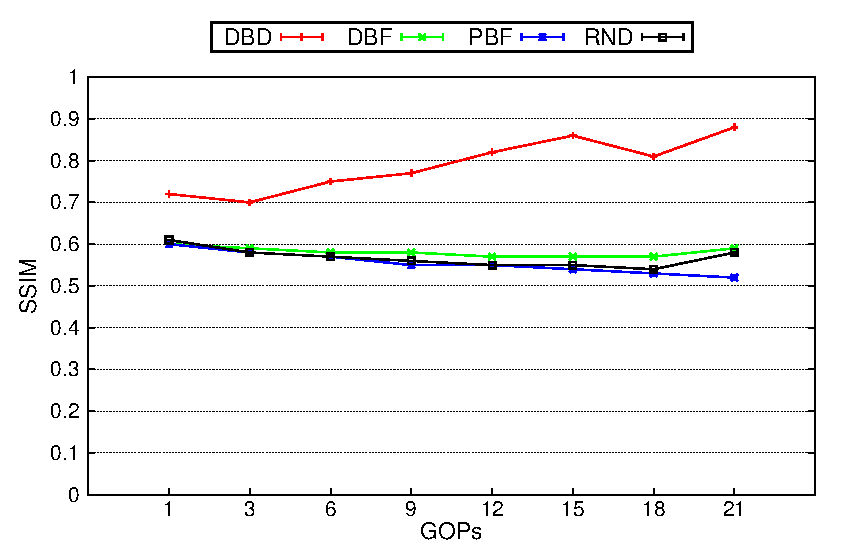
\includegraphics[width=.9\columnwidth]{./fig/selected/LineSSIMxGOPIDfinal.eps}
\caption{Average SSIM per GoP ID}
\label{fig:SSIM}
\end{center}
\end{figure}


Figure \ref{fig:SSIM2} demonstrates the SSIM of all forwarding schemes and for all scenarios when the density is of 400 vehicle/Km. The SSIM results reveal that DBD aims to transmit video sequences with a good quality level, where the average SSIM for all scenarios is 0.79. This means that the decoded videos have a high correlation with the original video flows. As an example, in scenarios with 200 nodes, the average SSIM is of 0.85, because less I frames were lost due to interferences or collisions.


\begin{figure}[tb]
\begin{center}
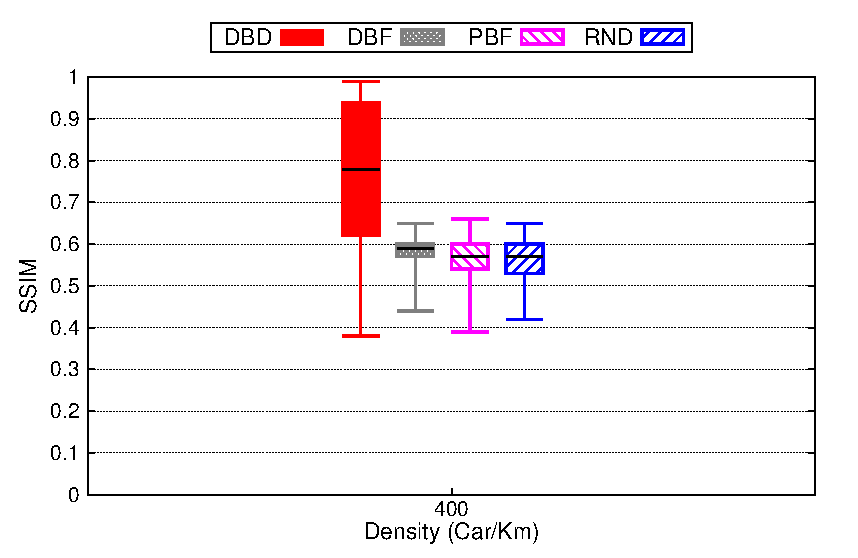
\includegraphics[width=.9\columnwidth]{./fig/selected/barSSIMxDen.eps}
\caption{SSIM values when the density is of 400 Car/Km}
\label{fig:SSIM2}
\end{center}
\end{figure}


Figure \ref{fig:SSIM3} shows SSIM results for video transmissions when ROI is 2 and 4 kilometres. In all the experiments, the results reveal that DBD aims to keep the SSIM for all video sequences around 0.82 and 0,72 when ROI = 2km and 4km, respectively. In dense scenarios, the number of collisions and interferences is high, which increases the number of frame losses. About 60\% of I frames were lost when DBF, PBF, and RND were responsible for forwarding packets. Without an I frame, the entire GoP cannot be decoded at the receiver side and the error propagates until the beginning of the next GoP, upon the reception of a new I frame.


\begin{figure}[tb]
\begin{center}
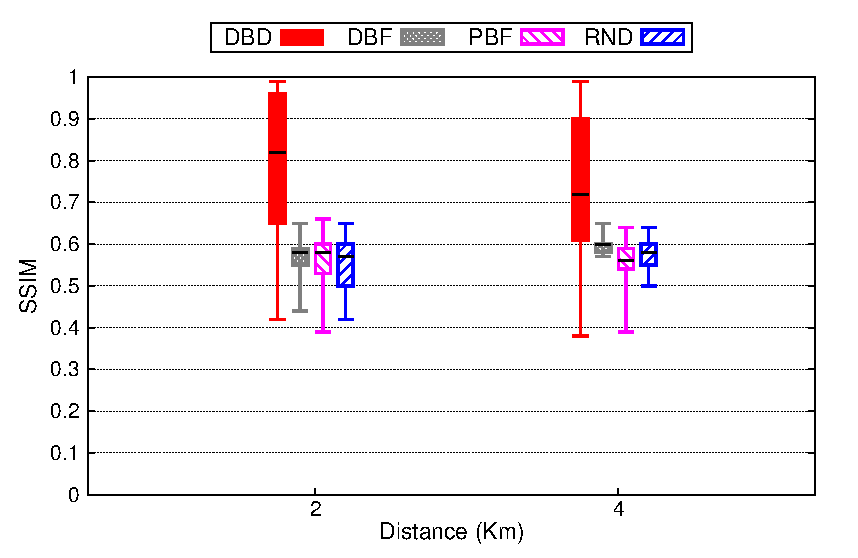
\includegraphics[width=.9\columnwidth]{./fig/selected/barSSIMxKm.eps}
\caption{SSIM values when the density is of 400 Car/Km}
\label{fig:SSIM3}
\end{center}
\end{figure}

Finally, we randomly selected video frames (GoP 15, 400 car/km, and $d(S,D)$ is of 2 km) with the aim of analyzing the frames from a user point-of-view, as displayed in Figure \ref{fig:POV}. When DBD is used to control the video transmission, it is possible to see that the frame quality is excellent. However, the quality level of the displayed frame when PBF, RND, and DBD are forwarding packets is not acceptable from the user point of view, that we can evaluate in a random frame at the receiver's side.


\begin{figure}[!t]
	\begin{center} \subfigure[DBD]{\label{fig:POVDBD}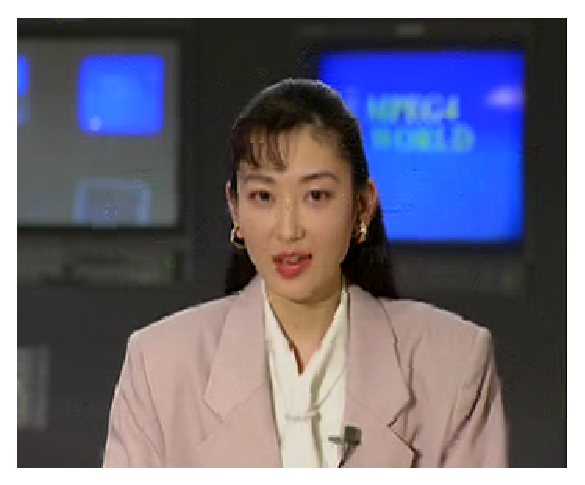
\includegraphics[width=.45\columnwidth]{./fig/frames/akiyo-Frame25-GOP15-DEN400-KM2-BITRATE1-MODEDBD-ST1-receiver.eps}}
    \subfigure[DBF]{\label{fig:POVDBF}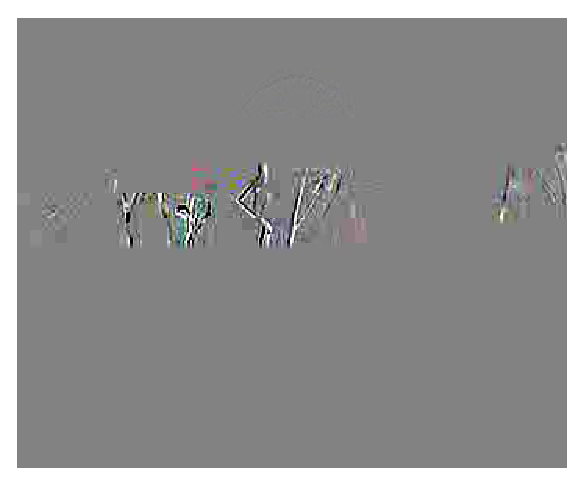
\includegraphics[width=.45\columnwidth]{./fig/frames/akiyo-Frame25-GOP15-DEN400-KM2-BITRATE1-MODEDBF-ST1-receiver.eps}}
    \subfigure[PBF]{\label{fig:POVPBF}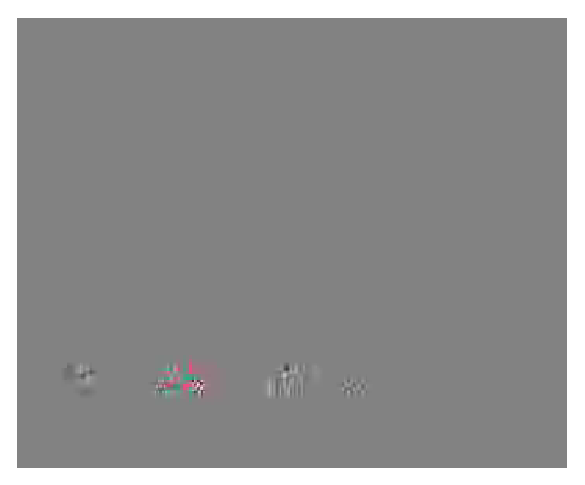
\includegraphics[width=.45\columnwidth]{./fig/frames/akiyo-Frame25-GOP15-DEN400-KM2-BITRATE1-MODEPBF-ST1-receiver.eps}}
    \subfigure[RND]{\label{fig:POVRND}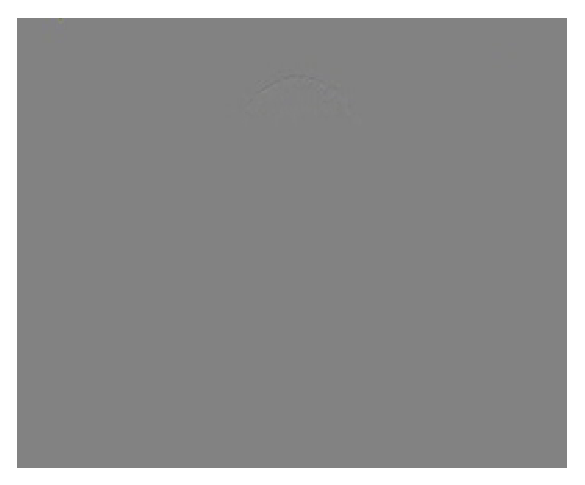
\includegraphics[width=.45\columnwidth]{./fig/frames/akiyo-Frame25-GOP15-DEN400-KM2-BITRATE1-MODERND-ST1-receiver.eps}}
	\caption{User point of view of one of the videos transmitted with the different routing protocols}
	\label{fig:POV}
	\end{center}
\end{figure}




\section{Conclusion}
\label{conclusion}
The paper presented a distributed application framework to share disaster/incident live videos with emergency vehicles, providing a QoE support in multi-hop high density highway scenarios.
Our main contributions are focused over 3 layers (application, routing and MAC) and may be summarized as follows: (a) the definition of the application layer automated framework for live video streaming; (b) the design and implementation of a beaconless multi-hop protocol that creates and maintains routes for real time data transmission; (c) the identification and elimination of the 802.11p MAC layer Spurious Forwarding problem through a loose cross-layer approach, without modifying the MAC layer itself; (d) the improvement of the overall network performance in terms of QoS (packet delivery ratio, delay, etc.) and QoE (SSIM), by showing the comparison of our relay scheme (DBD) with other ones, like DBF, PBD and RND.
Our simulations show an improvement of 30\% in terms of QoE and even more in terms of QoS by using our DBD protocol, compared to other protocols like DBF, PBF and RND, with very dense scenarios (compatible with car accidents) of 400 veh/km.
%The simulation results highlighted the benefits of DBD in sharing live videos flows. We measured the quality level of the video flows by means of a well-known metric for QoE, namely SSIM. Compared to DBF, PBF, and RND, DBD increases the SSIM values of received videos in about 30\% for scenarios with 400 vehicles/Km.

\section*{Acknowledgment}
E. Cerqueira is supported by The National Council for Scientific and Technological Development (CNPq) and Fundacao Amazonia Paraense de Amparo a Pesquisa (FAPESPA).


%
% The following two commands are all you need in the
% initial runs of your .tex file to
% produce the bibliography for the citations in your paper.
\bibliographystyle{abbrv}
\bibliography{bibliomultimedia}  % sigproc.bib is the name of the Bibliography in this case
% You must have a proper ".bib" file
%  and remember to run:
% latex bibtex latex latex
% to resolve all references
%
% ACM needs 'a single self-contained file'!
%
%APPENDICES are optional
%\balancecolumns

\balancecolumns
% That's all folks!
\end{document}
